%%%%%%%%%%%%%%%%%%%%%%%%%%%%%%%%%%%%%%%%%
% Arsclassica Article
% LaTeX Template
% Version 1.1 (1/8/17)
%
% This template has been downloaded from:
% http://www.LaTeXTemplates.com
%
% Original author:
% Lorenzo Pantieri (http://www.lorenzopantieri.net) with extensive modifications by:
% Vel (vel@latextemplates.com)
%
% License:
% CC BY-NC-SA 3.0 (http://creativecommons.org/licenses/by-nc-sa/3.0/)
%
%%%%%%%%%%%%%%%%%%%%%%%%%%%%%%%%%%%%%%%%%


%----------------------------------------------------------------------------------------
%	PACKAGES AND OTHER DOCUMENT CONFIGURATIONS
%----------------------------------------------------------------------------------------

\documentclass[
10pt, % Main document font size
a4paper, % Paper type, use 'letterpaper' for US Letter paper
oneside, % One page layout (no page indentation)
%twoside, % Two page layout (page indentation for binding and different headers)
headinclude,footinclude, % Extra spacing for the header and footer
BCOR5mm, % Binding correction
]{scrartcl}

%%%%%%%%%%%%%%%%%%%%%%%%%%%%%%%%%%%%%%%%%
% Arsclassica Article
% Structure Specification File
%
% This file has been downloaded from:
% http://www.LaTeXTemplates.com
%
% Original author:
% Lorenzo Pantieri (http://www.lorenzopantieri.net) with extensive modifications by:
% Vel (vel@latextemplates.com)
%
% License:
% CC BY-NC-SA 3.0 (http://creativecommons.org/licenses/by-nc-sa/3.0/)
%
%%%%%%%%%%%%%%%%%%%%%%%%%%%%%%%%%%%%%%%%%

%----------------------------------------------------------------------------------------
%	REQUIRED PACKAGES
%----------------------------------------------------------------------------------------

\usepackage[
nochapters, % Turn off chapters since this is an article        
beramono, % Use the Bera Mono font for monospaced text (\texttt)
eulermath,% Use the Euler font for mathematics
pdfspacing, % Makes use of pdftex’ letter spacing capabilities via the microtype package
dottedtoc % Dotted lines leading to the page numbers in the table of contents
]{classicthesis} % The layout is based on the Classic Thesis style

\usepackage{arsclassica} % Modifies the Classic Thesis package

\usepackage[T1]{fontenc} % Use 8-bit encoding that has 256 glyphs

\usepackage[utf8]{inputenc} % Required for including letters with accents

\usepackage{graphicx} % Required for including images
\graphicspath{{Figures/}} % Set the default folder for images

\usepackage{enumitem} % Required for manipulating the whitespace between and within lists

\usepackage{lipsum} % Used for inserting dummy 'Lorem ipsum' text into the template

\usepackage{subfig} % Required for creating figures with multiple parts (subfigures)

\usepackage{amsmath,amssymb,amsthm} % For including math equations, theorems, symbols, etc

\usepackage{varioref} % More descriptive referencing

%----------------------------------------------------------------------------------------
%	THEOREM STYLES
%---------------------------------------------------------------------------------------

\theoremstyle{definition} % Define theorem styles here based on the definition style (used for definitions and examples)
\newtheorem{definition}{Definition}

\theoremstyle{plain} % Define theorem styles here based on the plain style (used for theorems, lemmas, propositions)
\newtheorem{theorem}{Theorem}

\theoremstyle{remark} % Define theorem styles here based on the remark style (used for remarks and notes)

%----------------------------------------------------------------------------------------
%	HYPERLINKS
%---------------------------------------------------------------------------------------

\hypersetup{
%draft, % Uncomment to remove all links (useful for printing in black and white)
colorlinks=true, breaklinks=true, bookmarks=true,bookmarksnumbered,
urlcolor=webbrown, linkcolor=RoyalBlue, citecolor=webgreen, % Link colors
pdftitle={}, % PDF title
pdfauthor={\textcopyright}, % PDF Author
pdfsubject={}, % PDF Subject
pdfkeywords={}, % PDF Keywords
pdfcreator={pdfLaTeX}, % PDF Creator
pdfproducer={LaTeX with hyperref and ClassicThesis} % PDF producer
} % Include the structure.tex file which specified the document structure and layout

\hyphenation{Fortran hy-phen-ation} % Specify custom hyphenation points in words with dashes where you would like hyphenation to occur, or alternatively, don't put any dashes in a word to stop hyphenation altogether

%----------------------------------------------------------------------------------------
%	TITLE AND AUTHOR(S)
%----------------------------------------------------------------------------------------

\title{\normalfont\spacedallcaps{Internship report}} % The article title

%\subtitle{Subtitle} % Uncomment to display a subtitle

\author{\spacedlowsmallcaps{Vincent RÉBISCOUL}} % The article author(s) - author affiliations need to be specified in the AUTHOR AFFILIATIONS block

\date{} % An optional date to appear under the author(s)

% ----------------------------------------------------------------------------------------

\usepackage{tikz}
\newcommand{\N}{\mathbb{N}}
\newcommand{\V}{\mathcal{V}}

\begin{document}

%----------------------------------------------------------------------------------------
%	HEADERS
%----------------------------------------------------------------------------------------

\renewcommand{\sectionmark}[1]{\markright{\spacedlowsmallcaps{#1}}} % The header for all pages (oneside) or for even pages (twoside)
%\renewcommand{\subsectionmark}[1]{\markright{\thesubsection~#1}} % Uncomment when using the twoside option - this modifies the header on odd pages
\lehead{\mbox{\llap{\small\thepage\kern1em\color{halfgray} \vline}\color{halfgray}\hspace{0.5em}\rightmark\hfil}} % The header style

\pagestyle{scrheadings} % Enable the headers specified in this block

%----------------------------------------------------------------------------------------
%	TABLE OF CONTENTS & LISTS OF FIGURES AND TABLES
%----------------------------------------------------------------------------------------

\maketitle % Print the title/author/date block

\setcounter{tocdepth}{2} % Set the depth of the table of contents to show sections and subsections only

\tableofcontents % Print the table of contents
\section*{Abstract}
I did my internship at the Inria Grenoble and the subject was:
\textit{"Optimisation avec incertitudes: application à la gestion
  énergétique"} and it lasted 6 weeks. My supervisor was Bruno Gaujal
from  Inria. Here, I will present what was the general problem. Then,
I will discuss what I have done, which was a generalization of the
problem.


\newpage % Start the article content on the second page, remove this if you have a longer abstract that goes onto the second page

\section{A presentation of the problem}
Nowadays, energy consumption is a major issue. Indeed, more power is
more heat which causes a shorter life for the hardware. Obviously,
electricity needs to be produced so it means more pollution, more
spendings for the energy provider, the cooling devices etc... This is
why my supervisor and some of his colleagues have worked on how to minimize the
energy consumption on a processor.

\subsection{A processor consumes energy}
Let say we have a processor that has to do some work. To do it,
the processor can choose several speeds, it can go fast, slow,
intermediate etc... The consumption of energy will depend on the speed
chosen by the processor and the choice of the right speed will be the
core of the problem.
Here, we suppose that energy is a convex function of
the speed, nthat means that if we want to minimize the energy
consumption, we want to use great speed as little as possible. Now, we
want to make a mathematical model of a processor that receives tasks
over time and executes them in time. We also want a model that works
online. It means that the jobs are not known in advance by the
processor. To do that, we are gonna use a Markov Decision Process to
minimize the expected energy consumption to choose the right
speed. Here, we study a case where the processor works until a time
$T\in\N$, in our model, the time will be a finite set of the form
$\{0,1,\dots,T\}$. To represent a job $j_i$, we will need a 3-tuple
$(a_i,s_i,d_i)$ with $a_i\in\N$ the arrival time, in other words, the
time when the processor learns the job $j_i$. $s_i\in\N$ is the
workload (the ``amount of work''). And $d_i\in\N$ is the deadline, it
means that the job $j_i$ has to be finished before $t=a_i+d_i$. In the
following graph, I have represented several jobs: on the x-coordinate
I put the interval in which the work has to be done and on the
y-coordinate I put the workload of the jobs. For example, $j_2$ has an
arrival time $a_2=2$, a workload $s_2=3$ and a deadline $d_2=4$. 

\begin{center}
  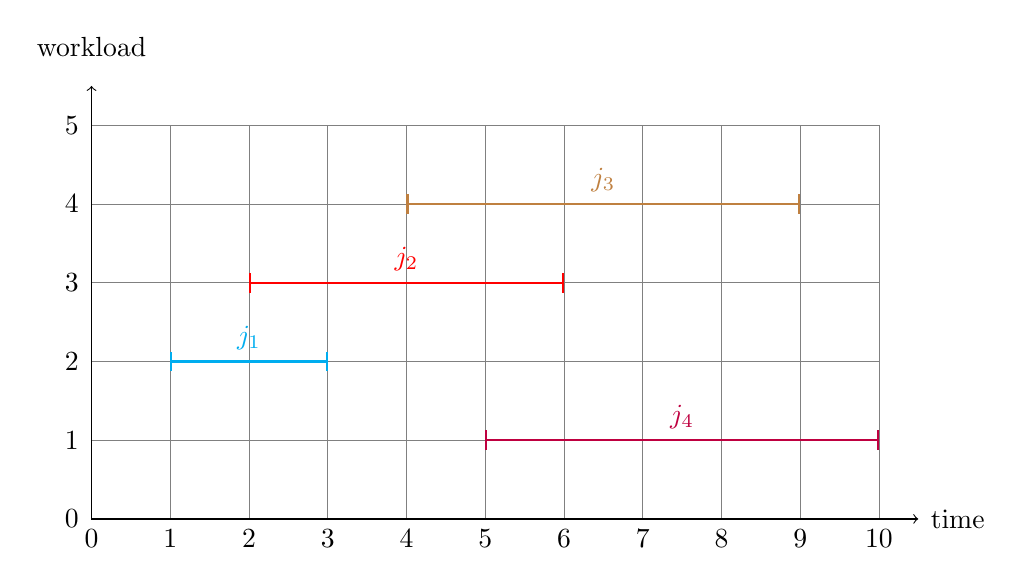
\begin{tikzpicture}
    \draw[help lines] (0,0) grid (10,5);
    \draw[<->] (0,5.5) -- (0,0) -- (10.5,0);
    \foreach \y in {0,1,...,5} \draw (-0.25,\y) node {\y};
    \foreach \x in {0,1,...,10} \draw (\x, -0.25) node {\x};
    \draw (11,0) node {time};
    \draw (0,6) node {workload};
    \draw[|-|,cyan,thick] (1,2) -- (3,2);
    \draw[cyan] (2,2.3) node {$j_1$};
    \draw[|-|,red,thick] (2,3) -- (6,3);
    \draw[red] (4,3.3) node {$j_2$};
    \draw[|-|,brown,thick] (4,4) -- (9,4);
    \draw[brown] (6.5,4.3) node {$j_3$};
    \draw[|-|,purple,thick] (5,1) -- (10,1);
    \draw[purple] (7.5,1.3) node {$j_4$};
  \end{tikzpicture}
\end{center}

We introduce two parameters: $D$ and $S$ which will be the maximal
deadline and the maximal workload. So, for any job
$j_i=(a_i,s_i,d_i)$ we have $s_i\leq S$, $d_i\leq D$.
The speeds that our processor can choose are represented by a finite
set $\V\subset\N$. To minimize the expected energy consumption, we
need to have some informations on the jobs that will come. We suppose
that we know $(\phi_{\sigma,\delta})_{0\leq\sigma\leq S,0\leq\delta\leq D}$ with
$\phi_{\sigma,\delta}$ being the probability that the job $j_i$
arriving at time $t$ has a deadline $d_i=\delta$ and a workload
$s_i=\sigma$. The fact that no job has arrived at time $t$ is
represented by a workload equals to zero.

\subsection{The remaining work function}



\end{document}